%
\begin{isabellebody}%
\setisabellecontext{thesis{\isacharunderscore}{\isadigit{5}}{\isacharunderscore}discussion}%
%
\isadelimtheory
%
\endisadelimtheory
%
\isatagtheory
%
\endisatagtheory
{\isafoldtheory}%
%
\isadelimtheory
%
\endisadelimtheory
%
\isadelimdocument
%
\endisadelimdocument
%
\isatagdocument
%
\isamarkupsection{Discussion\label{discussion}%
}
\isamarkuptrue%
%
\isamarkupsubsection{Automated Moral Agents in Practice \label{aiethics}%
}
\isamarkuptrue%
%
\endisatagdocument
{\isafolddocument}%
%
\isadelimdocument
%
\endisadelimdocument
%
\begin{isamarkuptext}%
In Chapter \ref{applications}, I demonstrated that my system is capable of performing sophisticated,
nuanced ethical reasoning. In this section and Section \label{computationalethics}, I outline how my
system could be used by AI agents and by human philosophers. My work on automating the categorical imperative 
could serve as one component of a partially or fully artificial ethical reasoner, or an ``ethical AI.''
Specifically, my system could be a categorical imperative library that takes as input the logical representation 
of a maxim and returns its moral status (if it is obligatory, prohibited, or permissible).

As it stands, my project can evaluate the moral status of maxims represented in my logic and potentially 
serves as one component of an ``ethics engine'' that an AI agent could use to make ethical decisions.
For example, my system could be combined with an input parser to translate moral dilemmas as represented 
to the AI agent into maxims in my logic. The ouput of my system could be fed into an output 
parser to translate this output into a prescription for the action the AI agent should take.
Figure \ref{fig:AIengine} depicts the workflow of this example ethics engine.%
\end{isamarkuptext}\isamarkuptrue%
%
\begin{figure}
\centering
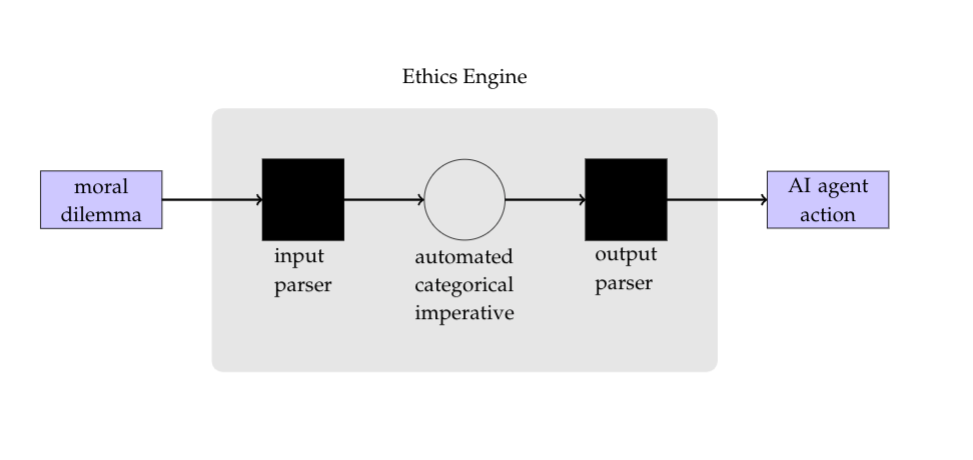
\includegraphics[scale=0.4]{AI_engine.png}
\caption{An example of an ethics engine for an artificial agent, which begins with a moral dilemma, 
passes it through an input parser, applies the automated Kantian ethics test, and then processes the 
output using an output parser. I contribute the automated Kantian ethics component.} \label{fig:AIengine}
\end{figure}
%
\begin{isamarkuptext}%
In this workflow, an AI agent is faced with a moral dilemma in some internal representation. The input
parser translates this internal representation into an appropriate logical representation, i.e. 
a circumstance, act, goal tuple. The output parser translates the output of the categorical imperative
library (the moral status of the maxim as obligatory, prohibited, or permissible) to a prescription for
action that the AI agent can act on. In order for my system to be used in an AI agent using the workflow
above, future work would need to develop such input and output parsers.%
\end{isamarkuptext}\isamarkuptrue%
%
\begin{isamarkuptext}%
The input parser must translate a complex real-world situation into a flat, logical representation. 
This requires that the input parser determine which circumstances are ``morally relevant''
for a maxim, a controversial judgement that requires commonsense reasoning.
There is robust debate in the literature on which circumstances should be considered when formulating a maxim. 
Some critics of Kant raise the ``tailoring objection,'' which is the worry that arbitrarily specific 
circumstances render any maxim universalizable. For example, the maxim ``When my name is Lavanya Singh 
and I am wearing a purple shirt and it is November 26th, I will lie in order to get some easy cash'' 
passes the universalizability test. Even if this maxim is willed universally, the circumstances are so 
specific that lying will not become the general mechanism for getting easy cash, so the lender will 
believe my lie and the maxim will remain effective. By tailoring the circumstances, any maxim can 
evade universalization.

The Kantian response to this criticism is to require that the circumstances included in the formulation
of the maxim be morally relevant. In the example above, my purple shirt and the date clearly have no bearing on 
the moral status of lying. On the other hand, consider the maxim, ``When I am unemployed, I will murder
someone in order to take their job.'' The circumstances of being unemployed clearly have some bearing on the moral
relevance of the murder in question; they speak to the motivation for the murder. While this view 
tracks how we actually perform moral reasoning, it raises the question of how we can determine
which circumstances are morally relevant. O'Niell answers this question by noting that the Formula of Universal Law is 
a ``test of moral worth rather than of outward rightness'' \citep[98]{constofreason}. The FUL is a way 
for an agent to decide how they should behave, not for a third-party to judge their behavior. Ethics is 
a personal process for Kant, so the FUL is designed to help agents internally make decisions, not to 
judge others' decisions. Because agents use the FUL to evaluate their own behavior, the test is at its 
best when they make a good faith effort to isolate the \emph{principle} of their action, rather than some
``surface intent'' \citep[87]{constofreason}. The FUL is supposed to determine if an agent's principle of action
is universally consistent, so it is most effective when an agent accurately formulates the principle
they act on. Circumstances are morally relevant if they accurately reflect the way that the agent is 
thinking about their own action. In the example above, the circumstance of wearing a purple shirt doesn't reflect
the principle of the liar's action. Its inclusion is clearly a disingenous attempt to evade the universalizability
test, but because the FUL is a test of personal integrity, it cannot withstand this kind of mental
gymnastics.

While this account of the formulation of a maxim describes how a well-intentioned human agent can determine 
morally relevant circumstances, the challenge remains open for automated ethics. In order for an automated
ethical agent to use the categorical imperative to its fullest extent, the input maxim fed into
my system or any automation of the FUL must be a good-faith attempt to capture the agent's principle
of action. However an action is turned into a maxim for my system to process, whether manually as I did
in Chapter \ref{applications} or using an automatic input parser, this transformation must be a good-faith 
attempt to capture the principle of action. 

Translating everyday situations into appropriate maxims is the bulk of the work that a Kantian human 
being does when making decisions. Common misconceptions about Kantian ethics\footnote{For example, critics 
of Kantian ethics worry that the maxim, ``When I am a
man, I will marry a man because I want to spend my life with him'' fails the universalizability
test because if all men only married men, sexual reproduction would stop. This argument implies 
that Kantian ethics is homophobic. Kantians often respond by arguing that the correct formulation of 
this maxim is, ``When I love a man, I will marry him because I want to spend my life with him,'' which
is universalizable because if everyone marries who they love, some men will marry women and others will
marry men.} often result from incorrectly formulated maxims, 
and the entire field of applied Kantian ethics is devoted to generating the right kinds of maxims to test. 

This representational question is one of the biggest challenges to using my categorical imperative library
in an AI ethics engine. One solution is for a human being to perform the role of the input
parser. Once an AI agent stumbles onto an ethical dilemma, a human being could take over, formulate 
the right question, and feed it into the categorical imperative library to see what action the categorical 
imperative would prescribe. For proponents of the ``human-in-the-loop'' model of AI ethics, in which 
ethical AI requires that humans guide machines \cite{loop}, this kind of human involvement may be a feature.
The outcome of the universalizability test will depend on how the human formulates the maxim; if the 
human puts garbage into the test, the test will return garbage out.

It is likely that, regardless of the strengths of the human-in-the-loop model, fully automated AI 
agents will exist. Even if developing this kind of AI is irresponsible,
such developments are likely and will require ethics engines, or risk no consideration of ethics at all. Even if 
AI without human supervision is scary, such AI with automated ethics is better than such AI without. 
In such a world, the input parser in my ethics engine would have to be automated. This would require 
that the parser translate the AI agent's internal representation to the appropriate logical representation. 
It is likely that, just as different implementations of automated ethics choose 
a particular ethical theory and implement it, different implementations of such an input parser would 
adopt different interpretations of commonsense reasoning and morally relevant circumstances. 

These interpretations of commonsense reasonining could inspire heuristics to classify circumstances as morally 
relevant. For example, one such attempt could define a moral closeness relation between an action, a 
goal, and circumstances. This heuristic could define morally relevant circumstances as those that 
reach a certain closeness threshhold with the action and the goal. Another possible heuristic could 
define some set of morally important entities, and classify morally relevant circumstances as those
that involve morally important entities. I discuss a potential machine-learning based approach which formulates
maxims based on a training set of appropriately formulated maxims in Section \ref{amapossible}.
Determining morally relevant circumstances, either using heuristics or human involvement, is a ripe 
area for future work.

Once the input has been parsed, either by a human or a machine, into  a sentence in my logic, my 
project can evaluate its moral status using my implementation of 
the FUL. Concretely, my project returns a value indicating if the maxim is obligatory, permissible, 
or prohibited. The maxim is prohibited if it fails the universalizability test, permissible if it passes, and obligatory 
if its negation fails the universalizability test. All three of these properties require testing if a 
certain theorem holds or not in my logic, a calculation that I demonstrate in Section \ref{testing}. 
Testing these properties requires that my system have a database of common sense or factual background. 
Different applications of my system may require different factual background (e.g. a self-driving car 
would need to know traffic regulations), so this common sense database may need to be application 
specific. As demonstrated in the examples in Chapter \ref{applications}, my system can produce sophisticated 
judgements with relatively little situational context. While the need for factual background is a challenge
for automated ethics, Chapter \ref{applications} demonstrates that it is less daunting than it seems. 

My system's output could be converted into some actionable, useful response with another output parser, 
and then passed back to the AI agent. For example, if the AI agent is equipped to evaluate natural 
language prescriptions, the status of the maxim could be parsed into a natural language sentence. The 
input parser, categorical imperative library, and output parser together constitute an ``ethics engine'' 
that AI developers could use as a black box implementation of an ethical theory. 

The ethics engine depicted above is a high-level example of one way to use my project to guide an artifical agent.
An automated version of the categorical imperative could become part of an ethics engine 
for an AI agent, with additional work to parse the input and the output. Effectively, the kind 
of automated ethics I implement could be a library that AI developers use to give AI agents the capacity for 
sophisticated ethical reasoning faithful to philosophical literature. This represents an improvement 
over existing AI ethics, which rarely attempts to capture the complexity 
of any ethical theory that philosophers plausibly defend.%
\end{isamarkuptext}\isamarkuptrue%
%
\isadelimdocument
%
\endisadelimdocument
%
\isatagdocument
%
\isamarkupsubsection{Computational Ethics \label{computationalethics}%
}
\isamarkuptrue%
%
\endisatagdocument
{\isafolddocument}%
%
\isadelimdocument
%
\endisadelimdocument
%
\begin{isamarkuptext}%
Above I explained how my system offers a mechanism for humans to build ethical AI agents. I also 
argue that computational ethics is a mechanism for computers to help humans think differently about 
philosophy. Just as theorem provers make mathematics more efficient and push mathematicians to think 
precisely about the phenomena they model, computational ethics can help philosophers think more precisely about 
philosophy. Below I share an example of the kind of philosophical insight that computational ethics 
can prompt and analyze the value that this tool offers to philosophers.%
\end{isamarkuptext}\isamarkuptrue%
%
\isadelimdocument
%
\endisadelimdocument
%
\isatagdocument
%
\isamarkupsubsubsection{Example of a Philosophical Insight: Well-Formed Maxims%
}
\isamarkuptrue%
%
\endisatagdocument
{\isafolddocument}%
%
\isadelimdocument
%
\endisadelimdocument
%
\begin{isamarkuptext}%
As presented in Section \ref{formalizingful}, in the process of developing my formalization of
the FUL, I discovered the certain kinds of maxims are badly formed, or inappropriate inputs to the 
universalizability test. The FUL is consistent only if it holds for ``well-formed maxims,''
such that neither the act nor goal are already achieved in the given circumstances. Precisely, 
a circumstance, act, goal tuple (c, a, g) is well-formed if $(\neg (c \longrightarrow a) ) \wedge 
(\neg(c \longrightarrow g))$. 

\noindent \textbf{Philosophical Implications of Badly-Formed Maxims}

Isabelle showed that the FUL can only hold for well-formed maxims logically, and I returned to Kantian
literature to better understand the philosophical implications of this idea. Because badly-formed maxims
neither change an agent's behavior nor generate meaningful obligations, they are not the right kinds of 
actions for practical reasoners to wonder about. They cannot be action-guiding and are thus not the kind of problem that 
ethics should be concerned with. Moreover, under the Kantian account of the will, the very act of asking 
if a badly-formed maxim is prohibited generates a contradiction by undermining the will's authority over itself. 

Consider the example badly-formed maxim, ``When eating breakfast, I will eat breakfast in order to 
eat breakfast.'' This maxim isn't clearly obligatory or prohibited, but there is something empty about 
it. Acting on this maxim could never result in any action. If an agent adopts this maxim, 
they decide that, in the circumstances ``eating breakfast'' they will perform the act ``eating breakfast''
for the purpose ``eating breakfast.'' In these circumstances, the act has 
already been performed! Adopting this maxim as a law to live by does not change how you live. If you adopt 
this maxim, when you are eating breakfast, you eat breakfast, but this statement is already tautologically true. 

Not only does a badly-formed maxim fail to prescribe action, any obligations or prohibitions it 
generates have already been fulfilled or violated. If a badly-formed maxim generates a prohibition, 
then this prohibition is impossible to obey, which is why my original version of the FUL was inconsistent. 
It is impossible to not eat breakfast while eating breakfast, because the circumstances assume that the 
act has happened. On the other hand, if a badly-formed maxim generates an obligation, then the obligation 
will have already been fulfilled. If you are required to eat breakfast while eating breakfast, then you've 
already fulfilled your obligation because the circumstances assume that the act has happened. Thus, 
a badly-formed maxim does not actually guide action because it doesn't generate new obligations or 
prohibitions. 

Because badly-formed maxims can't prescribe or alter action, they are not practically action-guiding and 
thus are not the right kinds of maxims for practical reasoners to evaluate. Insofar as ethics 
is supposed to guide action, badly-formed maxims cannot be part of this project because they
have no bearing on what someone should do. Practical reason is the kind of reason that helps us decide 
what we should do. A practical reasoner asks moral questions not as a mental puzzle or out of curiosity, but 
in order to decide how to act. A badly-formed maxim can never be action-guiding because it prescribes no new
actions or obligations. It is not the kind of maxim that a practical reasoner should consider, because it
will have no bearing on what the agent should do. There is no explicit prohibition against a badly-formed maxim 
like the breakfast example above, but it is the wrong kind of question for a practical reasoner to ask. 

Kantians can make an even stronger claim about badly-formed maxims—because maxims are laws that you 
give to yourself, asking if you should will a maxim as you will it undermines your will's law-giving 
ability. The circumstances of a badly-formed maxim assume that the agent has willed the maxim. Under 
the Kantian acount of willing, willing a maxim is equivalent to giving the maxim to yourself as a law. 
When you will a maxim, you commit yourself to the maxim's end. You cannot simultaneously 
commit yourself to a maxim and ask if you should be committing to it. To will the maxim is to adopt it as 
law—so the question, ``should I be willing this?'' is paradoxical. Either you haven't actually made 
the maxim your law (and thus haven't yet committed yourself to it), or you aren't actually asking 
the question (because the decision has already been made). Because a maxim is a law that you give to 
yourself, you cannot question it absent a sufficient reason (such as a change in the circumstances). 
To question a law arbitrarily is to not regard it as a law at all. This kind of questioning amounts to 
questioning the will's authority over itself, but this is impossible. The will definitionally has authority 
over itself, for that is what it is to be a will. 

A skeptic may argue that we do often ask ``should I be doing this?'' as we do something. 
Can this kind of question ever be valid? To understand this worry, I consider the maxim, 
``When dancing, I should just dance for the sake of dancing.'' While this maxim appears to be badly-formed (the 
circumstance ``dancing'' implies the act and goal of dancing), it is a question that practical reasoners 
do ask. I argue that the correct interpretation of this maxim is no longer a badly-formed maxim.

Under one reading of this maxim, ``I should just dance'' is referring to a different act than the 
circumstance ``when dancing''. The circumstance ``when dancing'' refers 
to rythmically moving your body to music, but ``I should just dance'' refers to dancing without anxiety, 
completely focused on the joy of dancing itself. More precisely, this maxim should read ``When 
dancing, I should abandon my anxiety and focus on dancing for the sake of dancing.'' This maxim when so 
modified is not vacuous at all—abandoning anxiety and focusing on dancing is an entirely different act 
from moving your body rythmically to music. This maxim is actually well-formed, and thus doesn't
pose a problem for my argument. It is entirely plausible to tell yourself ``When I am dancing, I should focus 
on dancing for the sake of dancing itself.'' The circumstances do not entail the act or the goal because 
they refer to different meanings of the word dancing. Any valid reading of this maxim will have the structure above, 
in which the act is actually different from the circumstances. A reasoner cannot accept their will 
as law-giving or commit themselves to an act and simultaneously question the act. Either they must be 
questioning a different act or they must have recieved new information to prompt the questioning, 
modifying the circumstances of the original maxim. 

Another related worry has to with maxims that we think are prohibited. Consider the maxim modified to 
read ``When dancing and seeing a child drowning, I should dance for the sake of dancing.'' Clearly this 
maxim is fit for moral evaluation, and we expect a moral theory to prohibit this maxim. The circumstances 
``When dancing and seeing a child drowning'' appear to entail the act of dancing, and the maxim thus 
appears badly-formed. Once again, this maxim is formulated incorrectly. In this case, the question 
that the agent is actually asking themselves is ``should I continue dancing?'' That is the 
maxim that they will adopt or reject. They want to know if they should stop dancing and go help the child. 
Dancing at the current moment and dancing at the next moment are different acts, and the circumstances 
imply the former but not the latter. A badly-formed maxim would have circumstances and act both 
``dancing at moment t,'' but this maxim has circumstances ``dancing at moment t'' and act ``dancing 
at moment t+1.''

\noindent \textbf{Implications for Self Doubt and Self Respect}

The idea that we cannot will badly formed maxims 

The dancing maxim can also be understood through the lens of self-doubt. Under this 
reading, the question ``When I am dancing, 
should I be dancing for the sake of dancing?" is the agent asking, ``Am I doing the right thing 
right now?" Unlike the drowning example, the agent is not asking about the next moment, but is expressing doubt about the 
moral validity of their behavior at this current moment. I do not want to argue that self-doubt always
 undermines the will—after all, self-doubt plays an important role in moral 
reasoning and is often the mark of a thoughtful agent. I argue instead that questions of self-doubt
do not actually involve vacuous maxims, for these are not the maxims that the agent is doubting. Indeed,
this example demonstrates that the tension between self-doubt and self-respect arises from a 
mistaken characterization of questions of self-doubt as questions about vacuous maxims.
I first explain the tension between self-doubt and self-respect in epistemology, then 
explain the parallel tension in ethics, and finally present a resolution of this tension.

In epistemology, there is a tension between the rational requirement to believe in yourself and the 
value of self-doubt, in moderation. Christensen presents the ``principle of self-respect," which requires 
that any rational agent refrain from believing that they have mistaken beliefs \cite[4]{christensen}. For example, I cannot 
rationally both believe that the sky is blue and believe that I believe that the sky is green. In other words, I cannot 
disapprove of my own credences. Christensen argues that this principle, which he abbreviates to SR, holds because 
a perfectly rational agent can make accurate and confident judgements about what they believe. If this 
is the case, violating SR results in a simple contradiction \cite[8-9]{christensen}. 

While most philosophers accept some version of SR\footnote{Van Fraassen, Vickers, Koons \cite[5]{christensen}}, 
Roush argues that the principle must be modified in order to account for healthy epistemic 
self-doubt. She argues that, while pathological second-guessing is roundly criticized, we are generally 
imperfect beings, and some sensitivity to our own limitations is a virtue \cite[2]{roushselfhelp}. Indeed, even Christensen 
acknowledges that total self-confidence is an epistemic flaw \cite[1]{christensen}. Thus, there is tension between the rational
requirement to respect our authority as believers and the practical reality that we are often wrong. 

This debate between self-respect and self-doubt in epistemology also applies to ethics. When we 
decide to act and commit ourselves to acting, we cannot simultaneously doubt the 
validity of our action. If human behavior is purposive, then the very act of committing oneself implies 
that one has sufficient reasons for committing oneself. These reasons may be flawed, but in making the 
commitment, the reasoner has accepted them. It is contradictory to claim that someone commits and questions 
simultaneously, because commitment itself implies a resolution to the question. Either the commitment 
is not real, or the question is not. I will call the principle that 
one cannot will a maxim and simultaneously question if they should will that maxim
``ethical self-respect" or ESR.

On the other hand, self-doubt is an important part of ethical reasoning. Just as believers are often 
mistaken, so are practical reasoners. An agent with perfect confidence, who is always sure that they 
are doing the right thing, is clearly not thinking deeply enough about their obligations. Some degree
of ethical self-doubt is normal and likely desirable. Thus, there is a tension between the rational
requirement of ESR and the intuitive validity of ethical self-doubt (ESD).

To resolve this tension, I return to my earlier example of a dancer. Imagine Sara is dancing at a 
weddding, when, in a moment of angst, she asks herself, ``Should I really be dancing right now?" 
What question is she asking here? The immediate answer is that she asking if the maxim, ``When dancing 
at your friend's wedding, dance for the sake of dancing" is a permissible maxim to act on. Notice that t
he maxim in question is vacuous: the circumstance ``when dancing at a friend's wedding" implies the act 
``dance." Because this is a vacuous maxim, it cannot be the maxim that she is questioning, for adopting 
this maxim could not have changed her behavior at all. Sara is asking a question about her actions and 
their validity. Any conclusions about the validity of a vacuous maxim would not help her, first because 
the maxim has no effect on her action, and second because any such validity would be a foregone conclusion
as she has already adopted the maxim. As 
I argued above, no practical reasoner can coherently ask themselves whether a vacuous maxim is 
valid or not without undermining their will, which is a contradiction. Thus, under 
the interpretation of self-doubt as a vacuous maxim, the tension between ESR and ethical self-doubt 
appears irresolvable. Those committed to this interpretation must abandon one principle or the other.

To resolve this issue, I turn to another interpretation of ethical self-doubt. Under this interpretation, 
when Sara asks, ``Should I really be dancing right now?" she wants to know if the maxim that 
resulted in the current moment when she is on the dance floor was actually 
the right thing to will. She is asking if she made the right 
decision in the past, when she decided to dance. The maxim that initiated the dancing would be something 
like ``When at a wedding, dance for the sake of dancing." This is the maxim that she is currently acting 
on, not the vacuous maxim ``When dancing, dance for the sake of dancing." Under this interpretation, 
there is no tension at all between self-doubt and self-respect. It is perfectly valid for a reasoner 
to doubt their prior moral judgements, just as it is perfectly rational for a believer to doubt their 
past beliefs \cite[3-4]{christensen}. Such doubt does not undermine the reasoner's decision-making 
capacity and is thus perfectly consistent with ethical self-respect. 

Not only does this second interpretation resolve the tension between ESR and ESD, it also more accurately 
tracks the operation of practical reason. As argued above, a practical reasoner would never ask themselves 
whether or not to will a vacuous maxim, because such a maxim would generate no meaningful obligations. 
Adopting such a maxim would not alter their behavior in any way. Moreover, the fact that a practical 
reasoner never adopts a vacuous maxim demonstrates the cause of the tension between ESR and ESD.
The tension itself arises from a misreading of questions of self-doubt as questions about 
the evaluation of vacuous maxims. A question of self-doubt cannot refer to a vacuous maxim and must 
instead refer to a well-formed maxim about the agent's past decision-making. As seen before, cases where 
agents appear to ask themselves about vacuous maxims are mistaken about the maxim in question, because 
such a question could never yield a useful answer for a practical reasoner. 



I arrived at this conclusion using Isabelle's proof-finding capabilities. Recall that Sledgehammer showed
that my original version of the FUL\footnote{The full logical representation is \isa{FUL{\isadigit{0}}\ {\isasymequiv}\ {\isasymforall}c\ a\ g\ s{\isachardot}\ not{\isacharunderscore}universalizable\ {\isacharparenleft}c{\isacharcomma}\ a{\isacharcomma}\ g{\isacharparenright}\ s\ {\isasymlongrightarrow}\ {\isasymTurnstile}prohibited\ {\isacharparenleft}c{\isacharcomma}\ a{\isacharcomma}\ g{\isacharparenright}\ s}.} contradicted
the axiom O\_diamond, which states that an obligated term cannot contradict its context\footnote{The 
full form of the axiom is $ O \{ A \vert B \} \longrightarrow \diamond (B \wedge A)$}. I hypothesized 
that there was some tension between the antecedent of the FUL, which states that all agents act on 
the maxim, and the consequent, which states that the maxim is prohibited. If the maxim has already 
been acted on, then not acting on it is impossible. Thus, the generated prohibition is impossible to 
obey, so the ought implies can principle and axiom O\_diamond are violated.

To test this hypothesis, I defined a specific maxim as a constant with no other defined features, 
and examined the consequences of the FUL holding for this specific maxim. Instead of quantifying over
all circumstance, act, goal tuples, I states that the FUL holds for the specific maxim defined by
by new constant. With this modification, Nitpick showed that the FUL is consistent! The reason that
the FUL could hold for a constant maxim but not for all maxims is that, as constants, the 
circumstances, act, and goal were all distinct. When they were quantified over, 
they could be identical. This motivated the definition of a well-formed maxim. 

To formalize this idea, I defined a maxim as \isa{well{\isacharunderscore}formed\ {\isasymequiv}\ {\isasymlambda}{\isacharparenleft}c{\isacharcomma}\ a{\isacharcomma}\ g{\isacharparenright}\ s\ w{\isachardot}\ {\isasymnot}\ c\isactrlbold {\isasymrightarrow}g\ w\ {\isasymand}\ {\isasymnot}\ c\isactrlbold {\isasymrightarrow}a\ s\ w}. In propositional
logic, a circumstance, act, goal tuple (c, a, g) is well-formed if $(\neg (c \longrightarrow a) ) \wedge 
(\neg(c \longrightarrow g))$. I tested my hypothesis by modifying my axiom to instead read $\forall$\emph{maxim
(maxim is well-formed} $\longrightarrow$ \emph{FUL holds for maxim}). This version of the FUL was indeed consistent!

To summarize, I realized that my initial attempt at formalizing the FUL was inconsistent because 
it required that the FUL hold for badly formed maxims, in which the circumstances entail the act or 
goal. The logical insight was that if FUL holds for maxims in which $(c \longrightarrow a) \vee 
(c \longrightarrow g)$, then the logic will be inconsistent.

SAY INCERDIBLE DIFFICULT WITHUT COMPUTER because computer looks for edge cases and makes assumptions precise.
it's an insight precisely because philosophers would never think of this edge case bc it's stupid.%
\end{isamarkuptext}\isamarkuptrue%
%
\isadelimdocument
%
\endisadelimdocument
%
\isatagdocument
%
\isamarkupsubsubsection{The Value of Computational Ethics%
}
\isamarkuptrue%
%
\endisatagdocument
{\isafolddocument}%
%
\isadelimdocument
%
\endisadelimdocument
%
\begin{isamarkuptext}%
I will now generalize from the personal insight reached above to the methodological value of 
computational ethics for philosophers.
I do not argue that computational ethics, as it stands today, uncovers philosophical insights that humans have not reached
or are incapable of reaching. After all, my understanding of a well-formed maxim could 
very well exist in the literature and certainly could be reached by a philosopher without any 
computational tools. Instead, I argue that computational tools prompt philosophers to ask questions that 
lead to insights. Philosophers already value precision, and the computer forces precision and makes formal
reasoning easier. Computational 
ethics can serve as another tool in a philosopher's arsenal, like a thought experiment or counterexample.
While the technology is not yet mature enough and easy enough to use to become widespread in philosophy
departments, technical progress could turn computational ethics into an easy-to-use tool for philosophers
that doesn't require any specialized progamming or logical knowledge.

The first contribution of computational ethics is precision \footnote{TODO: this article discusses 
benefits of precision: bookmarked}. Much of analytic philosophy involves 
making a particular concept precise. Thought experiments, arguments, counterexamples, and examples 
illustrate features of a concept in the hope of making the concept itself more precise. Computational 
ethics can help philosophers reach this goal of precision in another, potentially easier, way. 
Representing a philosophical idea in logic and implementing it in an interactive theorem prover requires 
making the idea precise to a degree that ordinary discussion can result in, but does not necessarily require. The initial representation 
of an idea in a logic requires making its form precise. For example, 
as I formalized the notion of a maxim, I had to understand its components and define it as a 
circumstance, act, goal tuple. Moreover, Isabelle's strict typing system required that I define 
coherent, consistent types for each of these entities and for a maxim as a whole. This requires understanding 
what role each of these components play in the FUL and assigning them each a type. In my example, I 
concluded that circumstances and goals are terms, which can be true or false at a world, and acts are 
open sentences, which are true for a particular subject at a particular world. This precision is possible 
without computational tools, but computational ethics forces a level of precision that ordinary discussion 
does not demand. Type fuzziness and overloaded definitions are all too common in philosophical writing and 
discussion (would be cool to cite some famous debate revolving around this idea), but computers don't 
allow this kind of imprecision.

Another, related benefit of computational ethics is that it makes formal ethics far less tedious. 
Certain subfields, such as philosophy of language, see such benefit in precision that they already 
use symbolic logic to represent philosophical concepts, just as mathematicians use symbolic logic to 
represent mathematical concepts. Some of this work requres tedious pencil and paper proofs to prove 
theorems, even when many of these theorems may not generate relevant philosophical insights. Interactive 
theorem provers make formal logic more accessible. Isabelle can complete a proof, starting from first principles, 
in a matter of seconds that would take a logician pages to complete. Similarly, Nitpick can generate 
examples or counterexamples to a proposition in a brute force manner. The computer can generate hypotheses
that philosophers can then think about, just as it did for me to prompt the insight above.

Just as calculators make arithmetic more accessible, computational ethics does the same for formal philosophy. 
Not all philosophy can or will 
be formalized or automated—after all, calculators didn't make accountants or mathematicians obsolete. Just as computers 
reduce the tedium in other aspects of our life, they can reduce the tedium involved in formal logic to 
allow mathematicians and philosophers to focus their attention on understanding.%
\end{isamarkuptext}\isamarkuptrue%
%
\isadelimdocument
%
\endisadelimdocument
%
\isatagdocument
%
\isamarkupsubsubsection{Looking Forward%
}
\isamarkuptrue%
%
\endisatagdocument
{\isafolddocument}%
%
\isadelimdocument
%
\endisadelimdocument
%
\begin{isamarkuptext}%
Computational ethics is at its infancy. The use of theorem provers in mathematics is just now beginning 
to make headway \cite{buzzardvideo}, even though theorem provers were first invented in the 1960's \cite{historyofITP}. In contrast, the first attempts to use theorem 
provers for ethics occurred in the last decade. The fact that this nascent technology is already 
helping humans reach non-trivial philosophical conclusions is reason to, at the very least, entertain 
the possibility of a future where computational ethics becomes as normal for philosophers.

To the skeptic, the ethical insights uncovered by the computer are not necessarily impressive 
philosophy. Indeed, the fact that a theorem prover requires specialized knowledge outside of the field 
of philosophy indicates that the technology is nowhere near ready for universal use in philosophy 
departments. However, history indicates that as computing power increases and computer scientists make 
progress, computational ethics will become more usable. Theorem provers in mathematics began as toys 
incapable of proving that the real number 2 is not equal to the real number 1, but Buzzard showed that 
moving from such a primitive system to a tool for Fields medal winning mathematics is possible in a 
matter of years \cite{buzzardvideo}. Countless examples from the history of computer science, from the Turing 
Test to AI game playing to protein folding, demonstrate that progress in computer science can make seemingly 
obscure computer programs useful and usable in ways that exceed our wildest imaginations. Indeed, 
programmable computers themselves initially began as unwieldy punch card readers, but their current ubiquity 
need not be stated. If computer scientists and philosophers invest in computational ethics, it can 
become as much a tool for philosophy as a calculator is for for arithmetic.\footnote{Is this too like, 
lalalala fantasy of computational philosophy? Would it be less so if I did more work explaining 
the history of theorem proving for math? Is this even that important for my project?}%
\end{isamarkuptext}\isamarkuptrue%
%
\isadelimdocument
%
\endisadelimdocument
%
\isatagdocument
%
\isamarkupsubsection{Theoretical Objections to Automating Kantian Ethics%
}
\isamarkuptrue%
%
\isamarkupsubsection{Related Work%
}
\isamarkuptrue%
%
\isamarkupsubsection{Conclusion%
}
\isamarkuptrue%
%
\endisatagdocument
{\isafolddocument}%
%
\isadelimdocument
%
\endisadelimdocument
%
\isadelimtheory
%
\endisadelimtheory
%
\isatagtheory
%
\endisatagtheory
{\isafoldtheory}%
%
\isadelimtheory
%
\endisadelimtheory
%
\end{isabellebody}%
\endinput
%:%file=~/Desktop/cs91r/paper/thesis_5_discussion.thy%:%
%:%24=6%:%
%:%28=8%:%
%:%40=10%:%
%:%41=11%:%
%:%42=12%:%
%:%43=13%:%
%:%44=14%:%
%:%45=15%:%
%:%46=16%:%
%:%47=17%:%
%:%48=18%:%
%:%49=19%:%
%:%50=20%:%
%:%51=21%:%
%:%52=22%:%
%:%55=26%:%
%:%56=27%:%
%:%57=28%:%
%:%58=29%:%
%:%59=30%:%
%:%60=31%:%
%:%61=32%:%
%:%64=34%:%
%:%65=35%:%
%:%66=36%:%
%:%67=37%:%
%:%68=38%:%
%:%69=39%:%
%:%73=41%:%
%:%74=42%:%
%:%75=43%:%
%:%76=44%:%
%:%77=45%:%
%:%78=46%:%
%:%79=47%:%
%:%80=48%:%
%:%81=49%:%
%:%82=50%:%
%:%83=51%:%
%:%84=52%:%
%:%85=53%:%
%:%86=54%:%
%:%87=55%:%
%:%88=56%:%
%:%89=57%:%
%:%90=58%:%
%:%91=59%:%
%:%92=60%:%
%:%93=61%:%
%:%94=62%:%
%:%95=63%:%
%:%96=64%:%
%:%97=65%:%
%:%98=66%:%
%:%99=67%:%
%:%100=68%:%
%:%101=69%:%
%:%102=70%:%
%:%103=71%:%
%:%104=72%:%
%:%105=73%:%
%:%106=74%:%
%:%107=75%:%
%:%108=76%:%
%:%109=77%:%
%:%110=78%:%
%:%111=79%:%
%:%112=80%:%
%:%113=81%:%
%:%114=82%:%
%:%115=83%:%
%:%116=84%:%
%:%117=85%:%
%:%118=86%:%
%:%119=87%:%
%:%120=88%:%
%:%121=89%:%
%:%122=90%:%
%:%123=91%:%
%:%124=92%:%
%:%125=93%:%
%:%126=94%:%
%:%127=95%:%
%:%128=96%:%
%:%129=97%:%
%:%130=98%:%
%:%131=99%:%
%:%132=100%:%
%:%133=101%:%
%:%134=102%:%
%:%135=103%:%
%:%136=104%:%
%:%137=105%:%
%:%138=106%:%
%:%139=107%:%
%:%140=108%:%
%:%141=109%:%
%:%142=110%:%
%:%143=111%:%
%:%144=112%:%
%:%145=113%:%
%:%146=114%:%
%:%147=115%:%
%:%148=116%:%
%:%149=117%:%
%:%150=118%:%
%:%151=119%:%
%:%152=120%:%
%:%153=121%:%
%:%154=122%:%
%:%155=123%:%
%:%156=124%:%
%:%157=125%:%
%:%158=126%:%
%:%159=127%:%
%:%160=128%:%
%:%161=129%:%
%:%162=130%:%
%:%163=131%:%
%:%164=132%:%
%:%165=133%:%
%:%166=134%:%
%:%167=135%:%
%:%168=136%:%
%:%169=137%:%
%:%170=138%:%
%:%171=139%:%
%:%172=140%:%
%:%173=141%:%
%:%174=142%:%
%:%175=143%:%
%:%176=144%:%
%:%177=145%:%
%:%178=146%:%
%:%187=148%:%
%:%199=150%:%
%:%200=151%:%
%:%201=152%:%
%:%202=153%:%
%:%203=154%:%
%:%204=155%:%
%:%213=157%:%
%:%225=159%:%
%:%226=160%:%
%:%227=161%:%
%:%228=162%:%
%:%229=163%:%
%:%230=164%:%
%:%231=165%:%
%:%232=166%:%
%:%233=167%:%
%:%234=168%:%
%:%235=169%:%
%:%236=170%:%
%:%237=171%:%
%:%238=172%:%
%:%239=173%:%
%:%240=174%:%
%:%241=175%:%
%:%242=176%:%
%:%243=177%:%
%:%244=178%:%
%:%245=179%:%
%:%246=180%:%
%:%247=181%:%
%:%248=182%:%
%:%249=183%:%
%:%250=184%:%
%:%251=185%:%
%:%252=186%:%
%:%253=187%:%
%:%254=188%:%
%:%255=189%:%
%:%256=190%:%
%:%257=191%:%
%:%258=192%:%
%:%259=193%:%
%:%260=194%:%
%:%261=195%:%
%:%262=196%:%
%:%263=197%:%
%:%264=198%:%
%:%265=199%:%
%:%266=200%:%
%:%267=201%:%
%:%268=202%:%
%:%269=203%:%
%:%270=204%:%
%:%271=205%:%
%:%272=206%:%
%:%273=207%:%
%:%274=208%:%
%:%275=209%:%
%:%276=210%:%
%:%277=211%:%
%:%278=212%:%
%:%279=213%:%
%:%280=214%:%
%:%281=215%:%
%:%282=216%:%
%:%283=217%:%
%:%284=218%:%
%:%285=219%:%
%:%286=220%:%
%:%287=221%:%
%:%288=222%:%
%:%289=223%:%
%:%290=224%:%
%:%291=225%:%
%:%292=226%:%
%:%293=227%:%
%:%294=228%:%
%:%295=229%:%
%:%296=230%:%
%:%297=231%:%
%:%298=232%:%
%:%299=233%:%
%:%300=234%:%
%:%301=235%:%
%:%302=236%:%
%:%303=237%:%
%:%304=238%:%
%:%305=239%:%
%:%306=240%:%
%:%307=241%:%
%:%308=242%:%
%:%309=243%:%
%:%310=244%:%
%:%311=245%:%
%:%312=246%:%
%:%313=247%:%
%:%314=248%:%
%:%315=249%:%
%:%316=250%:%
%:%317=251%:%
%:%318=252%:%
%:%319=253%:%
%:%320=254%:%
%:%321=255%:%
%:%322=256%:%
%:%323=257%:%
%:%324=258%:%
%:%325=259%:%
%:%326=260%:%
%:%327=261%:%
%:%328=262%:%
%:%329=263%:%
%:%330=264%:%
%:%331=265%:%
%:%332=266%:%
%:%333=267%:%
%:%334=268%:%
%:%335=269%:%
%:%336=270%:%
%:%337=271%:%
%:%338=272%:%
%:%339=273%:%
%:%340=274%:%
%:%341=275%:%
%:%342=276%:%
%:%343=277%:%
%:%344=278%:%
%:%345=279%:%
%:%346=280%:%
%:%347=281%:%
%:%348=282%:%
%:%349=283%:%
%:%350=284%:%
%:%351=285%:%
%:%352=286%:%
%:%353=287%:%
%:%354=288%:%
%:%355=289%:%
%:%356=290%:%
%:%357=291%:%
%:%358=292%:%
%:%359=293%:%
%:%360=294%:%
%:%361=295%:%
%:%362=296%:%
%:%363=297%:%
%:%364=298%:%
%:%365=299%:%
%:%366=300%:%
%:%367=301%:%
%:%368=302%:%
%:%369=303%:%
%:%370=304%:%
%:%371=305%:%
%:%372=306%:%
%:%373=307%:%
%:%374=308%:%
%:%375=309%:%
%:%376=310%:%
%:%377=311%:%
%:%378=312%:%
%:%379=313%:%
%:%380=314%:%
%:%381=315%:%
%:%382=316%:%
%:%383=317%:%
%:%384=318%:%
%:%385=319%:%
%:%386=320%:%
%:%387=321%:%
%:%388=322%:%
%:%389=323%:%
%:%390=324%:%
%:%391=325%:%
%:%392=326%:%
%:%393=327%:%
%:%394=328%:%
%:%395=329%:%
%:%396=330%:%
%:%397=331%:%
%:%398=332%:%
%:%399=333%:%
%:%400=334%:%
%:%401=335%:%
%:%402=336%:%
%:%403=337%:%
%:%404=338%:%
%:%405=339%:%
%:%406=340%:%
%:%407=341%:%
%:%408=342%:%
%:%409=343%:%
%:%410=344%:%
%:%411=345%:%
%:%412=346%:%
%:%413=347%:%
%:%414=348%:%
%:%415=349%:%
%:%416=350%:%
%:%417=351%:%
%:%418=352%:%
%:%419=353%:%
%:%420=354%:%
%:%421=355%:%
%:%422=356%:%
%:%423=357%:%
%:%424=358%:%
%:%425=359%:%
%:%426=360%:%
%:%427=361%:%
%:%428=362%:%
%:%429=363%:%
%:%430=364%:%
%:%431=365%:%
%:%432=366%:%
%:%441=371%:%
%:%453=373%:%
%:%454=374%:%
%:%455=375%:%
%:%456=376%:%
%:%457=377%:%
%:%458=378%:%
%:%459=379%:%
%:%460=380%:%
%:%461=381%:%
%:%462=382%:%
%:%463=383%:%
%:%464=384%:%
%:%465=385%:%
%:%466=386%:%
%:%467=387%:%
%:%468=388%:%
%:%469=389%:%
%:%470=390%:%
%:%471=391%:%
%:%472=392%:%
%:%473=393%:%
%:%474=394%:%
%:%475=395%:%
%:%476=396%:%
%:%477=397%:%
%:%478=398%:%
%:%479=399%:%
%:%480=400%:%
%:%481=401%:%
%:%482=402%:%
%:%483=403%:%
%:%484=404%:%
%:%485=405%:%
%:%486=406%:%
%:%487=407%:%
%:%488=408%:%
%:%489=409%:%
%:%490=410%:%
%:%491=411%:%
%:%492=412%:%
%:%493=413%:%
%:%494=414%:%
%:%495=415%:%
%:%496=416%:%
%:%497=417%:%
%:%498=418%:%
%:%499=419%:%
%:%508=422%:%
%:%520=425%:%
%:%521=426%:%
%:%522=427%:%
%:%523=428%:%
%:%524=429%:%
%:%525=430%:%
%:%526=431%:%
%:%527=432%:%
%:%528=433%:%
%:%529=434%:%
%:%530=435%:%
%:%531=436%:%
%:%532=437%:%
%:%533=438%:%
%:%534=439%:%
%:%535=440%:%
%:%536=441%:%
%:%537=442%:%
%:%538=443%:%
%:%539=444%:%
%:%540=445%:%
%:%549=448%:%
%:%553=450%:%
%:%557=452%:%